\documentclass[11pt]{beamer}
\usepackage[utf8]{inputenc}
\usepackage[T1]{fontenc}

% Remove these 2 lines
\usepackage[english]{babel}
\usepackage{blindtext}

% Defining a color
\usepackage{xcolor}
\definecolor{uwo-purple}{HTML}{4F2683}
\definecolor{uwo-gray}{HTML}{807F83}

\usetheme{CambridgeUS}

% Customizing the template
\setbeamercolor{frametitle}{fg=uwo-purple}
\setbeamercolor{title}{fg=uwo-purple}
\setbeamercolor{palette primary}{fg=black, bg=uwo-purple!30!white}
\setbeamercolor{palette secondary}{fg=black, bg=uwo-purple!20!white}
\setbeamercolor{palette tertiary}{bg=uwo-purple}


\begin{document}
	\author{Amir Haghighati}
	\title{Tweetycs}
	\subtitle{Understanding Real-Time Discussion of Health Issues on Twitter Through Visual Analytics (Ongoing Project)}
	\logo{
\includegraphics[width=1cm]{resources/uwo-purple.png}}
	\institute{Insight Lab}
	\date{April 10, 2019}
	\subject{UWORCS 2019}
	%\setbeamercovered{transparent}
	%\setbeamertemplate{navigation symbols}{}
	\begin{frame}
	\maketitle
	\centering\tiny\hyperlink{mailto:ahaghig3@uwo.ca}{ahaghig3@uwo.ca}
\end{frame}

\section*{Overview}
\begin{frame}
\frametitle{Agenda}
\tableofcontents
\end{frame}

\section{Introduction}
\subsection{Why Social Media?}
\begin{frame}
\frametitle{Social Media Usage}
	\begin{itemize}
		\item<1-> People gather \textcolor{blue}{health information} from diverse mediums, including \textcolor{uwo-purple}{social media}.
		\item<2-> Social media allows us to \textcolor{purple}{explore conversations} in a \textcolor{red}{rapid fashion}.
		\item<3-> \textcolor{cyan}{Twitter} is one of the largest social media platforms with \textcolor{blue}{more than 300 million} monthly active users.
		\item<4-> The \textcolor{teal}{unrestricted access} to opinions and \textcolor{teal}{large user base} has made Twitter a source for the collection and dissemination of information for various domains including \textcolor{blue}{health}.	
	\end{itemize}
\end{frame}

\begin{frame}
\frametitle{Social Media Usage (Cont'd)}
	\begin{itemize}
		\item<1-> Health organizations are using social media to:
		\begin{itemize}
			\item promote healthy lifestyle choices,
			\item identify disease outbreaks,
			\item explore human behaviour, and
			\item assess the public's perception of health issues
		\end{itemize}
		\item<2-> Individuals, news organizations, businesses, interest groups, and other groups also discuss health on Twitter.
	\end{itemize}
\end{frame}

\subsection{Challenges}
\begin{frame}
\frametitle{Challenges of Social Media}
	\begin{itemize}
		\item<1-> On any given day, \textcolor{red}{over 500 million tweets} are posted.
		\item<2-> The \textcolor{uwo-purple}{sheer number} of tweets, variety in \textcolor{blue}{quality of information}, and \textcolor{brown}{identity of user accounts} makes it \textcolor{red}{harder} to analyze public discourse on Twitter.
		\item<3-> There exist challenges for the public to improve their knowledge on a \textcolor{cyan}{wide variety} of health issues on Twitter.
		\begin{itemize}
			\item<4-> Following a particular health organization may be	beneficial for learning about a specific health hazard.
			\item<5-> Obtaining a \textcolor{teal}{high-level understanding} of social discourse on a wide variety of health issues, remains a challenge.
		\end{itemize}
	\end{itemize}
\end{frame}

\subsection{Opportunities}
\begin{frame}
\frametitle{What is The Purpose of Utilizing Social Media?}
\framesubtitle{For Understanding Public Discourse}
\begin{itemize}
	\item<2-> A high-level understanding can:
	\begin{enumerate}
		\item help addressing \textcolor{blue}{misinformation}
		\item equip individuals with a better \textcolor{teal}{mental structure}
	\end{enumerate}
	to assess how health issues are discussed.
	\item<3-> Health professionals and social scientists can use this lens to:
	\begin{enumerate}
		\item better \textcolor{cyan}{understand} public perception of health issues and
		\item determine how to better utilize Twitter for \textcolor{uwo-purple}{health promotion}
	\end{enumerate}
\end{itemize}
\end{frame}

\section{Background}
\subsection{Existing Research}
\begin{frame}
\frametitle{Existing Research}
	\begin{itemize}
		\item<1->Previously, a combination of \textcolor{cyan}{manual content annotation} and \textcolor{brown}{computational models} have been used to analyze the \textcolor{red}{sentiment} of discourse of health issues (e.g., marijuana usage, perception of H1N1 vaccine).
		\begin{itemize}
			\item<2->Sentiment analysis is concerned with the use NLP and computational linguistics to identify and extract \textcolor{red}{subjective information} from human language.
		\end{itemize}
		\item<3->Some existing works also used machine learning techniques to \textcolor{blue}{classify} tweets based on user description, genre, theme, and relevance to the topic of discussion (e.g., e-cigarettes, breast-cancer, dental pain).
		\item<4-> Existing research has focused predominantly on understanding \textcolor{red}{one or two} health topics.
		
	\end{itemize}
\end{frame}

\subsection{Analysis}
\begin{frame}
\frametitle{Our Aim}
\framesubtitle{What can we do?}
	\begin{itemize}
		\item<1-> Existing research has focused predominantly on understanding \textcolor{red}{one or two} health topics.
		\item<2-> Building a tool to provide insight into a \textcolor{blue}{variety of health issues} is possible through a \textcolor{brown}{visual analytic} perspective.
		\begin{itemize}
			\item<3-> Visual Analytics (VA) enhances the understanding of data by combining computational models and techniques (e.g., machine learning techniques) with interactive visualizations.
			\item<4-> Visual Analytics $\neq$ some charts!
		\end{itemize}
		\item<5-> But how can we combine machine learning with visualization and interaction?
	\end{itemize}
\end{frame}

\begin{frame}
\frametitle{Our Aim (Cont'd)}
\framesubtitle{Questions We Want to Answer}
\begin{itemize}
	\item Who talks about what?
	\item Is there a theme for these discussions? How many themes are out there?
	\item What is purpose of these discussions?
	\item Is there any relationship between a specific health issue and the sentiments from different sides of the discussions (e.g., media corporations and government officials)?
	\item ...!?
\end{itemize}
\end{frame}

\section{Proposed Method}
\subsection{Part One: Non Real-Time Analysis}
\begin{frame}
\frametitle{Part One}
\framesubtitle{Data Collection}
\begin{itemize}
	\item<1-> Using Tweepy (a Twitter API) and \textcolor{red}{117} search terms, a collection of \textcolor{red}{535,973} unique English language tweets over a 1 month period was curated.
	\begin{itemize}
		\item<2-> Search terms: causes identified by the Institute for Health Metrics and Evaluation (IHME)
		\item<3-> Metadata about the tweeter (account description, number of followers and following accounts, verification status) was also retrieved.
	\end{itemize}
	\item<4-> Retrieved data was stored in a MongoDB database.
\end{itemize}
\end{frame}

\begin{frame}
\frametitle{Part One (Cont'd)}
\framesubtitle{Analysis - Sentiment and Categories}
\begin{itemize}
	\item<1-> Initially, AlchemyAPI (now acquired by IBM) was used for sentiment analysis: each tweet got a sentiment score in the range (-1,1).
	\item<2-> Based on previous research and an analysis of 500 sample tweets:
	\begin{itemize}
		\item five content themes:
		\begin{enumerate}
			\item Educational
			\item Fundraising
			\item Personal
			\item Promotional
			\item Unrelated
		\end{enumerate}
		\item<3-> and six user categories:
		\begin{enumerate}
			\item Businesses
			\item Celebrities
			\item Interest Groups
			\item Media
			\item Official Agencies
			\item General Public
		\end{enumerate}
	\end{itemize}
\end{itemize}
\end{frame}

\begin{frame}
\frametitle{Part One (Cont'd)}
\framesubtitle{Analysis - Model Construction and Model Selection}
\begin{itemize}
	\item<1-> Classification of tweets and the users into the specified categories was done by variations in classification techniques:\\
	Toggling the inclusion of a specific feature in training models using bag of words and linear support vector classifiers.
	\item<2-> Taking only \textit{`description'} of the tweeter into consideration and running 100 experiments on 3000 labeld tweets (20:80 - train:test)\\
	$\rightarrow Average Accuracy Rate =$ \textcolor{red}{86.86\%} in classifying \textcolor{cyan}{users}.
	\item<3-> Taking \textit{`text'}, \textit{`count of keywords'}, and \textit{`user verification status'} of the tweets into consideration and running 100 experiments on the same set\\
	$\rightarrow Average Accuracy Rate =$ \textcolor{red}{81.44\%} in classifying \textcolor{cyan}{tweets}.
	\item<4-> Removing unrelated tweets $\rightarrow$ \textcolor{red}{416,900} tweets remained.
\end{itemize}
\end{frame}

\begin{frame}
\frametitle{Part One (Cont'd)}
\framesubtitle{Visualization}
	\begin{figure}
		\centering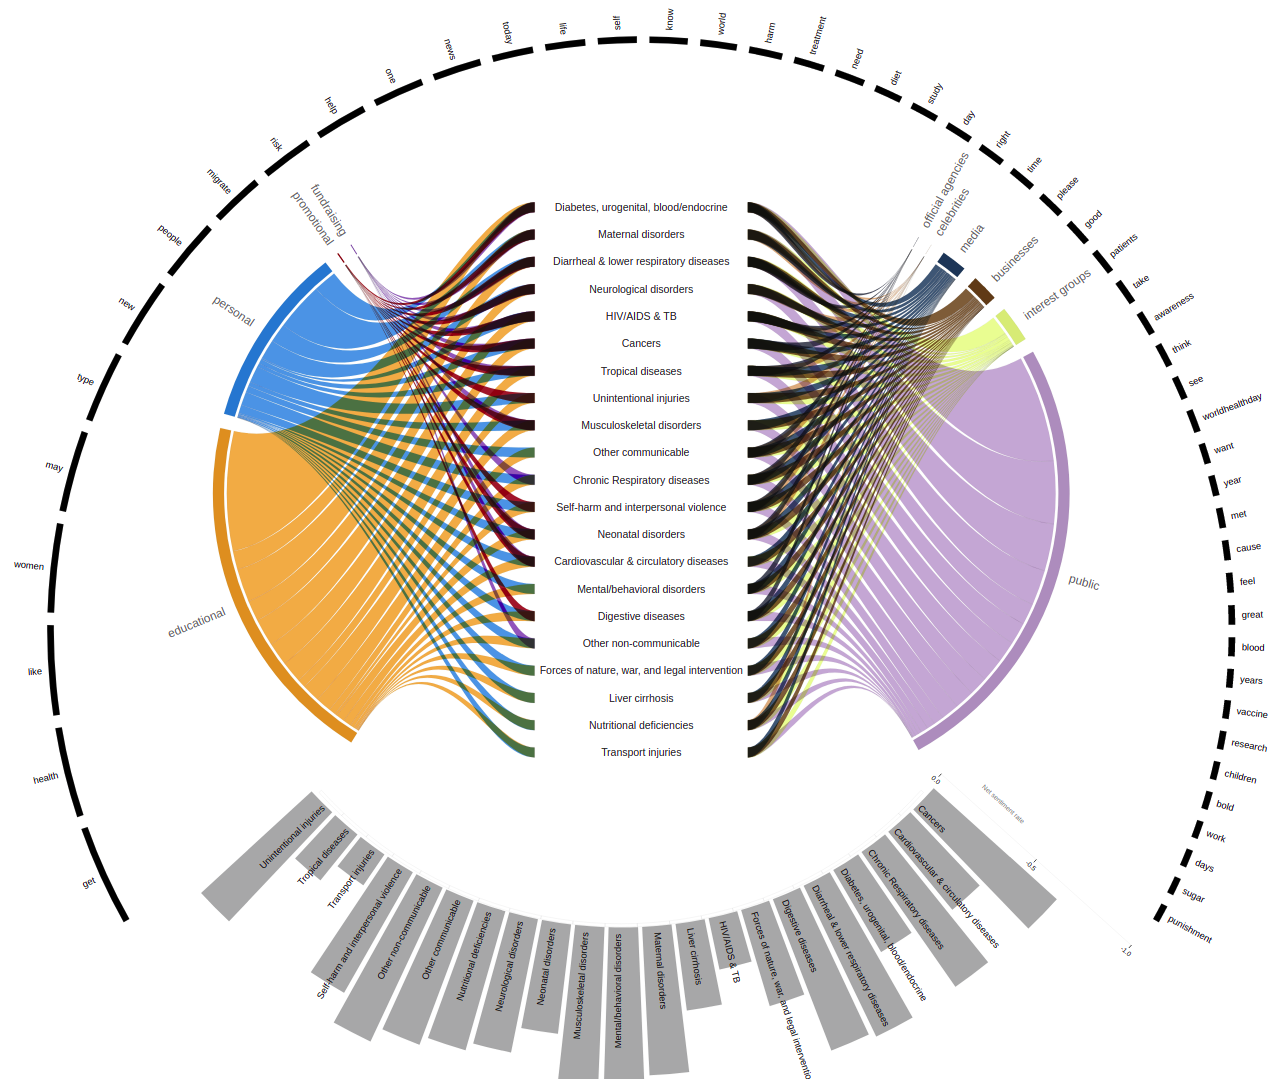
\includegraphics[width=8.5cm]{resources/config.png}
	\end{figure}
\end{frame}

\subsection{Part Two: Real-Time Visual Analytics}
\begin{frame}
\frametitle{Part Two}
\framesubtitle{Where is The Analytics?}
	\begin{itemize}
		\item<1-> Different supervised/unsupervised ML techniques $\rightarrow$ Different utility for each user
		\item<2-> Online streams of tweets $\rightarrow$ Need for stream processing and asyncronous programming
		\item<3-> Different possibilities for users $\rightarrow$ Customized utilities through interaction with ML techniques and visualizations
		\item<4-> Increasing \textcolor{red}{epistemic utility} for the user in order to understand the public discourse in the context of his/her interest.
	\end{itemize}
\end{frame}

\begin{frame}
\frametitle{Part Two (Cont'd)}
\framesubtitle{Ongoing Framework}
\begin{itemize}
	\item A Python API is subscribing to streams and saving the tweets in the database.
	\item The API incorporates several machine learning techniques and these techniques are being executed with respect to the old data and the new incoming chunks of data.
	\item The user who is interacting with the Visualization will receive the updates on tweets and would be given the option of choosing the result of different ML techniques.
\end{itemize}
\begin{figure}
	\centering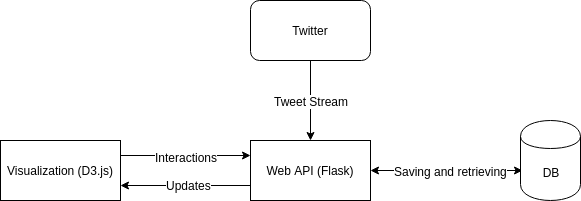
\includegraphics[width=6cm]{resources/UWORCS2019.png}
\end{figure}
\end{frame}

\begin{frame}
\frametitle{Thank you!}
	Questions?
\end{frame}

\section*{Backup Slides}
\begin{frame}
\frametitle{Accuracy Rate for User Category Model Construction}
	\begin{table}[]
		\begin{tabular}{|l|c|}
			\hline
			Model & Avg. Acc. Rate (\%) \\ \hline
			A1: description & 86.86 \\ \hline
			B1: description + screen name & 79.83 \\ \hline
			C1: description + name + influence score & 79.84 \\ \hline
			D1: description + name + influence score + verified & 79.75 \\ \hline
		\end{tabular}
	\end{table}
\end{frame}

\begin{frame}
\frametitle{ Accuracy Rate for Tweet Theme Model Construction}
\begin{table}[]
	\begin{tabular}{|l|c|}
		\hline
		Model & Avg. Acc. Rate (\%) \\ \hline
		A2: tweet & 80.99 \\ \hline
		B2: tweet + reserved keywords & 81.09 \\ \hline
		C2: tweet + verified & 81.14 \\ \hline
		D2: tweet + reserved keywords + verified & 81.44 \\ \hline
	\end{tabular}
\end{table}
\end{frame}
\end{document}